\usetikzlibrary{arrows.meta}


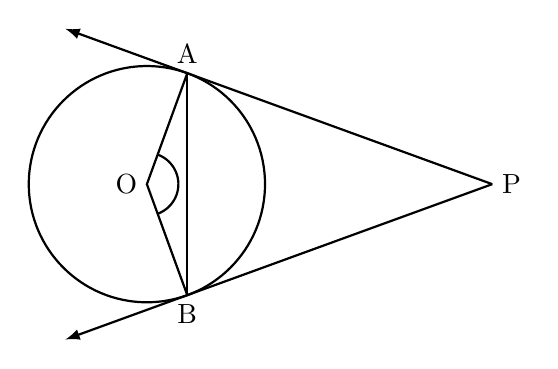
\begin{tikzpicture}[scale=1]

  % Define the center of the circle
  \coordinate (O) at (0,0);

  % Define the radius
  \def\R{1.5}

  % Draw the circle
  \draw[thick] (O) circle (\R);

  % Define points A and B on the circle using exact polar coordinates
  \coordinate (A) at (70:\R);
  \coordinate (B) at (-70:\R);

  % Define point P outside the circle mathematically so PA and PB are exact tangents.
  % Since OAP is a right triangle, OP = R / cos(70)
  \coordinate (P) at ({1.5/cos(70)}, 0);

  % Extend the tangent lines past A and B for the arrows.
  % Using 'pos=1.4' creates a coordinate exactly on the line PA/PB, extended 40% further.
  \path (P) -- (A) coordinate[pos=1.4] (EndA);
  \path (P) -- (B) coordinate[pos=1.4] (EndB);
  
  % Draw the tangent lines starting from P, passing exactly through A and B, ending with arrows
  \draw[thick, ->, >=latex] (P) -- (EndA);
  \draw[thick, ->, >=latex] (P) -- (EndB);

  % Draw the lines connecting O, A, B
  \draw[thick] (A) -- (O) -- (B);
  \draw[thick] (A) -- (B);

  % Add labels for the points exactly where they appear
  \node[left] at (O) {O};
  \node[above] at (A) {A};
  \node[below] at (B) {B};
  \node[right] at (P) {P};

  % Add an arc for angle AOB exactly centered on O
  % We use relative positioning '++(angle:radius)' to start the arc exactly on line OB
  \draw[thick] (O) ++(-70:0.4) arc (-70:70:0.4);

\end{tikzpicture}